\documentclass[12pt,a4paper]{article}
\usepackage[utf8]{inputenc}
\usepackage[english]{babel}
\usepackage{amsmath}
\usepackage{amsfonts}
\usepackage{amssymb}
\usepackage{algorithm}
\usepackage{algorithmicx}
\usepackage{algpseudocode}
\usepackage{tabularx}
\usepackage{multirow}
\usepackage{graphicx}
\usepackage{cite}
\usepackage[left=2cm,right=2cm,top=2cm,bottom=2cm]{geometry}
%\usepackage[headsepline, manualmark]{scrlayer-scrpage}
%\clearpairofpagesstyles

\makeatletter
\def\fps@figure{htbp}
\makeatother

\author{\\Research Project\\ \\Thomas Schick\\Florian Soulier\\ \\ Institute for Information Technology\\
Cologne University of Applied Sciences}
\title{Reinforcement Learning Agents for StarCraft II}
\begin{document}
\maketitle
\pagenumbering{Roman}
\newpage
\tableofcontents{}
\newpage
\pagenumbering{arabic}
\section{Introduction} 
When talking about artifical intelligence the most brought up topics often are recognition of images or sound based on vast amounts of correctly labeled data.
These technology rely heavily on human input to label the data in order for the machine learning algorithm to learn on.
The ability to learn abstract concepts however, differs strongly from the sheer memorizing of certain values in a pixels greyscale brightness.
This ability to learn is arguably one of, or even the most crucial aspect of human intelligence. And this is where reinforcement learning comes into play.
In this field of artifical intelligence, we attempt to guide an agent by supervisory signals in the form of rewards and penalties to learn an optimal behavior.
In the recent past a lot of milestones for reinforcement learning have been reached. The researchers at DeepMind aswell as @TODO
This work is motivated by the leaping steps the technology has made.
We adjusted the scope of the problem to a something we though to be reasonable when considering the time and resources available for this research project. 
This project contributes to to deep reinforcement learning research by asssessing hyperparameters and models to state-of-the-art algorithms.
\section{Artifical Neural Networks}
This section describes the basics of simple neural networks. Since biological neural networks are the role model for the structure of so called artifical neural networks (ANN), some information about them will be presented first.
Following up with an overview on the internal functionality of artifical neurons, the smallest component of ANNs.
In order to store large amounts of information, such as memories of events, artificial neural networks can be used. Their structure and functions are modelled on those of biological neural networks, however greatly simplified.
Each 
Artifical neuronal networks can be an equivalent model to the turing machine, regarding computability.
\subsection{The Biological Paradigm}
The mammal brain combined with the nervous system and it's capabilities in information processing serve as an archetype for today's artificial neural networks\cite{Rojas1996}
The fundamental components of such biological systems are neurons, complex and very small cells, which react to electrochemical signals.
The human nervous system, for example, consists of up to $10^{12}$ interconnected neurons.
Although, there are different types of neurons they share some basic characteristics. As shown in \ref{fig:neuron_schemantic} a neuron consists of a cell body with the nucleus, dendrites to receive stimuli of other cells and an axon ending with synapses used to pass on an electrical signal \cite{Patterson1997}.
\begin{figure}
    \centering
    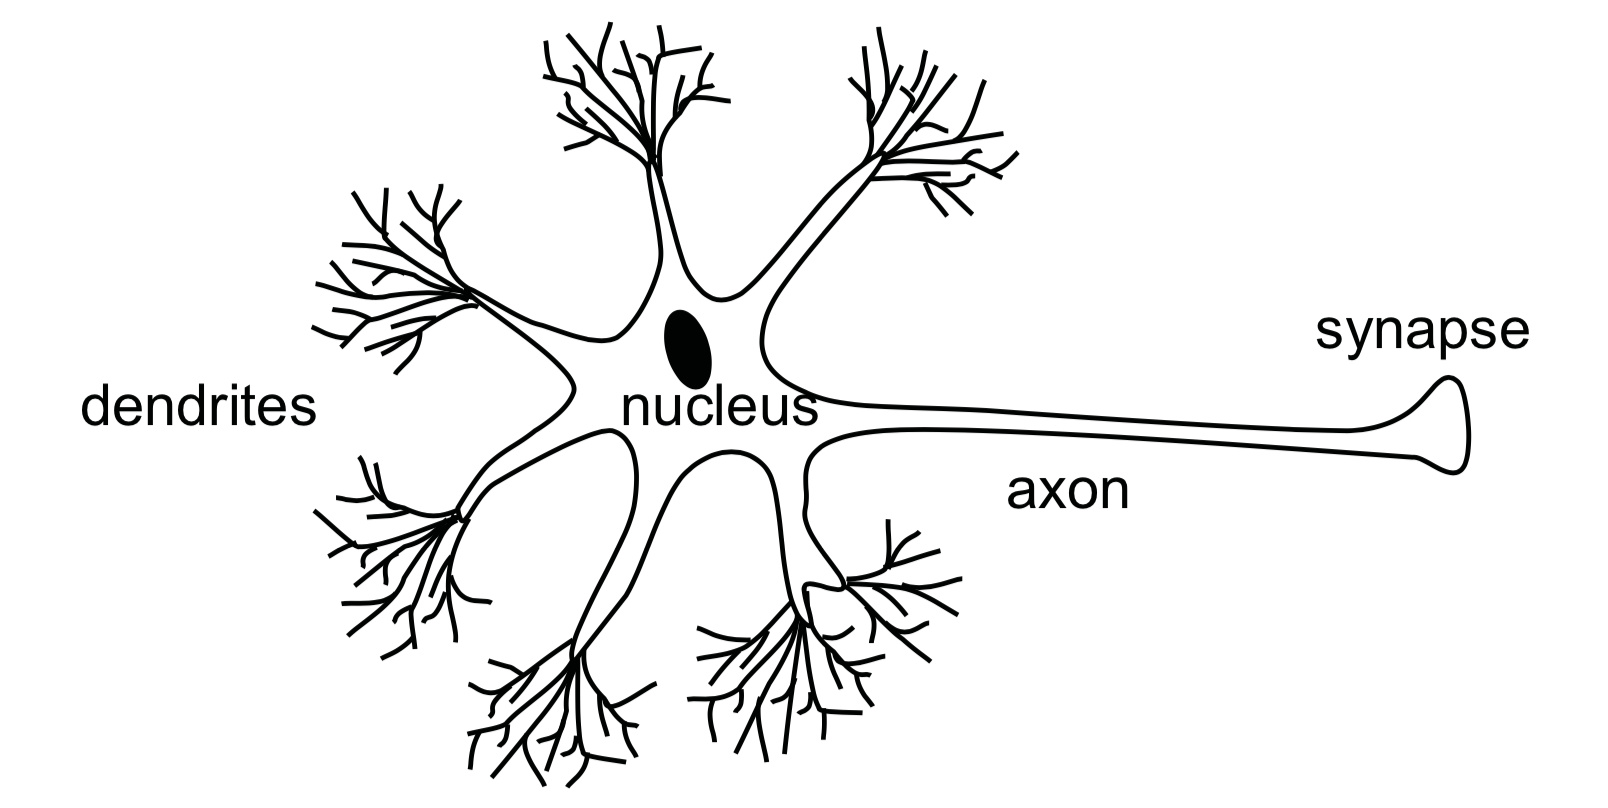
\includegraphics[width=0.5\linewidth]{Figures/Neuron_schemantic_depiction.png}
    \caption{Schemantic depiction of a neuron}
    \label{fig:neuron_schemantic}
\end{figure}
A neuron receives electrochemical stimuli from other neurons or receptors, which act as biological sensors.
As a result of stimulation, the neuron fires a short sequence of electrical pulses via the axon to the synapses in order to stimulate other neurons or actor cells like the muscles. On single neuron can be connected to a thousand other neurons. Due to different types of synapses the signals at the transition can either be amplified or weakened \cite{Patterson1997}.
Nowadays the synapses in the neural network are seen as the main storage for information, so considered to be the main location of knowledge\cite{Rojas1996}.
\subsection{Artifical Neurons}
After a crude explanation of the biological mechanisms inside a neuron, we will now have a look at the technical imitation. A simple model of an artificial neuron also denoted as a processing unit can be seen as a three-stage system with multiple inputs and one single output (see fig.\ref{fig:artifical_neuron}).
\newline
Thereby, the inputs $x_i$ mimic the biological structure of dendrites. By applying weights $w_i$, which can either have positive or negative values, to every external input-signal they represent the capability of synapses to amplify or weaken the signals. The input values, as well as the output values,  can be real, binary or bipolar \cite{Patterson1997}.
\begin{figure}
    \centering
    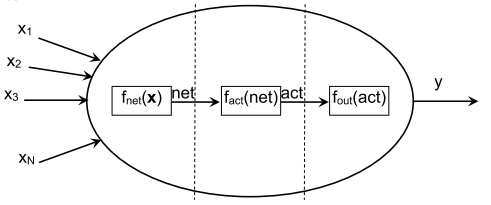
\includegraphics[width=0.5\linewidth]{Figures/artificial_neuron.png}
    \caption{Three stage model of an artifical neuron \cite{Bartz2018}.}
    \label{fig:artifical_neuron}
\end{figure}
\newline
In the first stage, the input stimuli of the neuron are combined into a so-called net-value. This net-value leads to a particular level of activity within the neuron. Although, for some classification tasks there are also other possibilities like distance from center \cite{Schwenker2001}, most times a weighted sum is used as a net function. In the definition of net sometimes a base level of excitation is stated, which is taken into account by a so-called bias value $\Theta$. To allow a compact notation this bias value is usually given as a fixed input value $x_0 = -1$ and a corresponding weight, so that $\Theta = -w_0$. The weighted sum can then be notated as:
\begin{equation}
    \label{eq:net}
    net = \sum_{n=0}^N\omega_n * x_n
\end{equation}
After multiple inputs are combined into a cumulative net value the next stage is the so-called activation function $f_{act}$. This function is normally a monotonously increasing function of net. Figure @todo shows some popular examples.

The third and last stage is the output function, which imitates the effects of the axon and the synaptic connection. This stage is very often neglected because the goal of the model is not to copy the biological behavior as accurately as possible but to provide a processing tool inspired by neural mechanisms. So the output value in most cases is the same as the activation value, it holds $y = act$. In this case, the output function is an identity function (see fig. @todo).
\subsection{Multi Layer Perceptron}
The most commonly used form of artifical neuronal networks is the form of a multi layer perceptron. The perceptron is the fundamental unit in deep learning models. It can perform a basic mathematical operation, more specifically it can linearly
combine a set of incoming values from it's inputs. The MLP features multiple layers of perceptrons, where each neuron is connected to all neurons of the following layer, forming a fully connected network.


\subsection{Activation Functions}
\subsection{Optimizing Neural Networks}
\section{Deep Learning}
Deep learning describes a set of machine learning methods for ANNs with multiple hidden layers. One can classify the learning methods of ANNs into three basic categories:  supervised learning, unsupervised learning, and reinforcement learning. Although this work concentrates on reinforcement learning, we will have a short look at the other two methods.
\subsection{Supervised Learning}
As the term supervised learning suggests, human supervision is necessary for the ANN to learn. In most cases, this means, that the training data has been labeled with human insight beforehand so that the samples contain both input and desired output values. During the learning process, the calculated output of the ANN is compared to the correctly labeled output of the sample, and an error or divergence is measured. This error is then used to adjust the connecting weights within the network. This way the network can achieve better performance and minimize the error in the next epoch of training. 
Training is considered successful, if the resulting error lies within an acceptable range, for all samples of the training dataset.
As of today, the most used algorithm for supervised learning is Backpropagation, implemented successfuly by Rumelhart in 1985 \cite{Rumelhart1985},{Patterson1997}.
\subsection{Unsupervised Learning}
Machine learning without known target values or rewards granted by the environment is generally defined as unsupervised learning. The learner tries to recognize patterns and statistical regularities that stand out from the amorphous noise. During training, the learner machine intensifies specific connection weights so that the results for the clustering of central, representative datasets match up \cite{Patterson1997}. Popular fields of use are automated clustering of data points or compressing data to achieve dimensional reduction.
\section{Deep Reinforcement Learning}
Machine learning as a field of science has been around for decades now. It is part of the overall field of artificial intelligence and enables systems to recognize patterns and regularities on the basis of datasets.
One could say knowledge is derived from experiences. So in Reinforcement Learning, like a human, the AI agent learns from the consequences of its actions, rather than being explicitly taught. This feedback loop is what reinforcement learning is about.
And it is on the rise. Most outstanding achievements in deep learning were made due to deep reinforcement learning. DeepMind's AI agents teach themselves how to walk, run and overcome obstacles.
Google's Alpha Go has beaten the world's best human player in the board game Go, Google's Alpha Star is reaching high levels of play in the
video game StarCraft II, the game which will be used for experiments in this project as well.
\newline
\begin{figure}
    \centering
    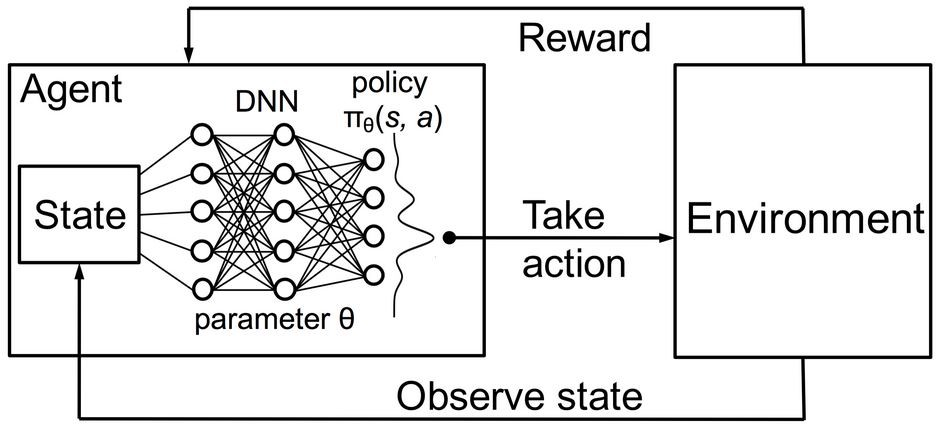
\includegraphics[width={0.5\linewidth}]{Figures/DRL_schemantic_depiction.jpeg}
    \caption{Schemantic depiction of a reinforcement learning process.}
    \label{fig:drl_schemantic}
\end{figure}
In Deep Reinforcement Learning, the Agent is represented by a neural network, which stores a representation of the experiences made in its environment. The agent observes the current state of the environment and decides which action to take from a pool of actions, called the action space.
The decision is made on the basis of the current state and past experiences. Based on the taken action, the environment occasionally provides the agent with a reward. The amount of reward determines the quality of the taken action with regards to solving the given problem.
The objective of an AI agent is to maximize the accumulated reward over time, by learning to take the right actions in any given circumstances.
However, the reward is mostly delayed, thus not instantaneous. This makes time play a fundamental role in reinforcement learning and the decision process it revolves around.
This decision process can be modeled as a Markov Decision Process, which will be covered in the next section.
\subsection{Markov Decision Process}
A Markov Decision Process (MDP) is a discrete time stochastic control process. MDP is the state of the art approach to model the complex environment of an AI agent. An MDP is defined by the tuple ${\{S, A, P, R, \gamma\}}$. A and S are finite sets of actions and states. P is a state transition probability matrix. R is the reward expected by the agent. In the following the MDP will be build up step by step. \newline
Every problem that the agent is supposed to solve can be considered as a sequence of states (a state may be for example a chess board configuration). While taking actions, the agent moves from one state to another. In a Markov Process, the current state depends only on the previous state. This is also called the Markov Property (\ref{eq:markov_prop}).
\begin{equation}
    \label{eq:markov_prop}
    P[S_{t+1}|S_t] = P[S_{t+1}|S_1,S_2,S_3,...,S-t]
\end{equation}
A Markov Process is a memoryless random process. It is a sequence of random states, with each state fulfilling the Markov property. This means that the probability distribution of the next state is fully determined by just the current state and not any other state. A transition happens with a certain probability ${Pss'}$
\begin{equation}
    \label{eq:trans_prob}
    Pss' = P[S_{t+1} = s' | S_t =s]
\end{equation}
The state transition matrix ${P}$ defines transition probabilities from all states $s$ to all successor states ${s'}$:
\begin{equation}
    \label{eq:trans_matrix}
    P = \begin{bmatrix}
        P_{11} & \dots & P_{1n}\\
        \vdots & \ddots & \vdots\\
        P_{n1} & \dots & P_{nn}\\
    \end{bmatrix}
\end{equation}
Now, in reinforcement learning, we add a reward function ${R}$ to the process.  ${R}$ defines the reward that the agent will receive at the next time step when being in state $s$ at time $t$:
\begin{equation}
    \label{eq:reward_func}
    R_s = \mathbb{E}[R_{t+1}|S_t = s]
\end{equation}
This way we get a Markov chain with values called a Markov Reward Process.
Since the Markov Process is a stochastic process, the reward given by the value function has to be seen as an expected reward.
 Reward, sticking to the chess game example, means certain states of the board are more promising than others in terms of the potential to win the game. After all, the total reward $G_t$(\ref{eq:markov_reward}), which is the expected accumulated reward across the sequence of all states.
\begin{equation}
    \label{eq:markov_reward}
    G_t = R_{t+1} + R_{t+2} + ... = \sum_{k=0}^\infty R_{t+k+1}
\end{equation}
 Every reward is weighted by the so-called discount factor $\gamma \in [0, 1]$, shown in \ref{eq:disc_markov_reward}.
 \begin{equation}
    \label{eq:disc_markov_reward}
    G_t = R_{t+1} + \gamma R_{t+2} + ... = \sum_{k=0}^\infty \gamma^kR_{t+k+1}
 \end{equation}
 The higher the factor, the less important are rewards that lie further into the future. This is beneficial, since immediate rewards may earn more interest than delayed and hence more uncertain rewards. Conveniently, it also helps to eliminate infinite returns in a cyclic Markov process.
These value of a state is defined by the value function ${v(s)}$, which gives the long-term value of a state $s$. Or in other words, it determines the amount of reward the agent can get starting in state $s$ until the process terminates:
\begin{equation}
    \label{eq:value_func}
    v(s) = \mathbb{E}[G_t|S_t =s]
\end{equation}
The value function can be decomposed into two parts: Immediate reward $R_{t+1}$ and the discounted value of successor state ${\gamma v(S_{t+1})}$. This way, one can concisely express the so-called Bellman equation using matrices and the column vector $v$, containing one entry per state from 1 to $n$:
\begin{equation*}
    v = R + \gamma Pv
\end{equation*}
\begin{equation}
    \label{eq:bellman_matrix}
    \begin{bmatrix}
        v(1)\\
        \vdots\\
        v(n)\\
    \end{bmatrix} = \begin{bmatrix}
        R_1\\
        \vdots\\
        R_n\\
    \end{bmatrix} + \gamma \begin{bmatrix}
        P_{11} & \dots & P_{1n}\\
        \vdots\\
        P_{n1} & \dots & P_{nn}\\
    \end{bmatrix}  
    \begin{bmatrix}
        v(1)\\
        \vdots\\
        v(n)\\
    \end{bmatrix}
\end{equation}
The Bellman equation (\ref{eq:bellman_matrix}) can be solved directly as it is a linear equation. However, as the complexity of the underlying Markov process increases, the problem becomes too big to be solved directly as the computational complexity for the Bellman equation is $O(n^3)$ for $n$ states.
\newline
Now in an MDP, the next state is not only dependent on the current state, but also on the action the agent takes in that state. Therefore, the taken action $a$ has to be added to (\ref{eq:trans_prob}) and (\ref{eq:reward_func}):
\begin{equation}
    \label{eq:trans_prob_with_action}
    P_{ss'}^a = P[S_{t+1} = s' | S_t =s, A_t = a]
\end{equation}
\begin{equation}
    \label{eq:reward_func_with_action}
    R_s^a = \mathbb{E}[R_{t+1}|S_t = s, A_t = a]
\end{equation}
The MDP describes the basis for an algorithm popularly used for reinforcement learning, called Q-Learning, which the next section will cover.
\subsection{Q-Learning}
Q-learning is an off-policy TD control algorithm that seeks to find the best action to take given the current state. It was invented by Christopher Watkins in 1989 and is defined by:
\begin{equation}
    \label{eq:q_learn}
    Q(S_t, A_t) \leftarrow Q(S_t, A_t) + \alpha [R_{t+1}+\gamma \max_aQ(S_{t+1},a)-Q(S_t,A-t)]
\end{equation}
It is considered off-policy because the q-learning function learns from actions that are outside the current policy, like taking random actions. More specifically, q-learning seeks to learn a policy that maximizes the total reward. It is making use of a model-free prediction and control methods.

In this case, the learned action-value function, Q, directly approximates q, the optimal
action-value function, independent of the policy being followed. The Q-value resembles the discounted value of a state-action pair. This dramatically
simplifies the analysis of the algorithm and enabled early convergence proofs. The policy however
still affects control because it determines which state-action pairs are visited and updated.
However, all that is required for correct convergence is that all pairs continue to be
updated. This is a minimal requirement in the sense that
any method guaranteed to find optimal behavior in the general case must require it.
Under this assumption and a variant of the usual stochastic approximation conditions on
the sequence of step-size parameters, Q has been shown to converge with probability 1 to
q. The Q-learning algorithm is shown below in the procedural form\cite{Sutton2015}:
\begin{algorithm}
    \caption{Q-learning for estimating a policy $\pi$}
    \begin{algorithmic}
    \State Algorithm parameters: step size $\alpha \in (0, 1]$, small  $\epsilon > 0$
    \State Initialize $Q(s,a)$, for all $s\in S^+$, $a\in A(s)$, arbitrarily except that $Q(terminal)=0$
    \State Loop for each episode:
    \While{$S$ is not terminal}
        \State Initialize $S$
        \ForAll{step of episode}
            \State Choose $A$ from $S$ using policy derived from $Q$ (e.g., $\epsilon$-greedy)
            \State Take action $A$, observe $R$, $S'$
            \State $Q(S, A) \leftarrow Q(S, A) + \alpha [R_{t+1}+\gamma \max_aQ(S_{t+1},a)-Q(S_t,A-t)]$
            \State $S \leftarrow S'$
        \EndFor
    \EndWhile
    \end{algorithmic}
\end{algorithm}

The following figure (\ref{fig:dql_procedure}) is a depiction of the Q-learning process for DQNs, using an online and a target network. It shows how the online DQN, given the current state $S_t$, predicts the values of actions. Then it selects the best action based on an $\epsilon$ greedy policy and observes the environment's reaction to the action taken. In the {\it collect experience} block, all observations from the environment are collected. Like the received rewards and the state, the agent ends up in.

\begin{figure}
    \centering
    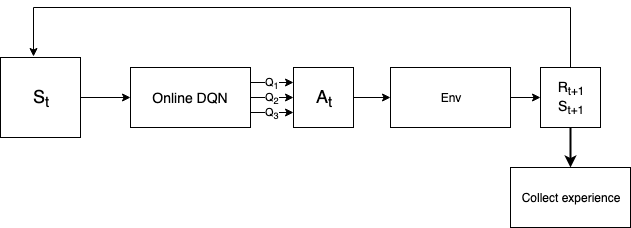
\includegraphics[width=0.8\linewidth]{Figures/QLearningProcedure.png}
    \caption{Deep Q-learning Procedure}
    \label{fig:dql_procedure}
\end{figure}
Once enough experience has been collected, one can start training the online neural network while keeping the target network fixed. After a set amount of steps, the weights of the two networks get synchronized. Minh et al \cite{Mnih2016} suggest selecting so-called mini-batches of size 32 from the pool of collected experiences for training. The following equation \ref{eq:exp_tuple} describes an experience tuple. It contains state, action, immediate reward, and the following state:

\begin{equation}
    \label{eq:exp_tuple}
    e_t = (s_t, a_t, r_{t+1}, s_{t+1})
\end{equation}

Equation \ref{eq:target_q_value} shows how the target Q-value can be calculated. From the experience, we already know the immediate reward $R_{t+1}$. Gamma ($\gamma$) is the discounting factor which is multiplied by the argmax of the Q-values predicted by the target DQN. In other words, the action with the highest predicted Q-value gets selected and discounted for the target Q-value.

\begin{equation}
    \label{eq:target_q_value}
    Y_t^{DQN} = R_{t+1} + \gamma * max_aQ'(a)
\end{equation}

One thing to note here is that at this stage we are using an untrained target DQN to predict the future rewards and select the maximum of its predictions. This is introducing a strong bias towards that maximum, a weakness of the Q-learning algorithm that is discussed in \ref{double_q_learning}. 

Having calculated the target Q-value, one can subtract the predicted Q-value for the action taken and thereby calculate the loss, see equation \ref{eq:loss_function}.
\begin{equation}
    \label{eq:loss_function}
    Loss = [Y_t^{DQN} - Q(A_t)]^2
\end{equation}
Using the gradient descent algorithm, one can now update the weights in the online DQN and repeat the process.

As proven by Hasselt, Guez, and Silver \cite{VanHasselt2015}, the Q-learning algorithm suffers from its argmax component overestimating action values. Thus, they introduced the Double Q-Learning method, which will be covered in the next section.
\subsection{Double-Q-Learning}\label{double_q_learning}
The max operator in standard Q-learning and DQN, in (2) and (3), uses the same values both to select and to evaluate an action. This makes it more likely to select over- estimated values, resulting in overoptimistic value estimates. To prevent this, we can decouple the selection from the evaluation. This is the idea behind Double Q-learning (van Hasselt, 2010). In the original Double Q-learning algorithm, two value functions are learned by assigning each experience randomly to up- date one of the two value functions, such that there are two sets of weights. For each update, one set of weights is used to determine the greedy policy and the other to determine its value. For a clear comparison, we can first untangle the selection and evaluation
\begin{algorithm}
    \caption{Double Q-learning}
    \begin{algorithmic}
    \State Algorithm parameters: step size $\alpha \in (0, 1]$, small  $\epsilon > 0$
    \State Initialize $Q(s,a)$, for all $s\in S^+$, $a\in A(s)$, arbitrarily except that $Q(terminal)=0$
    \State Loop for each episode:
    \While{$S$ is not terminal}
        \State Initialize $S$
        \ForAll{step of episode}
            \State Choose $A$ from $S$ using policy derived from $Q$ (e.g., $\epsilon$-greedy)
            \State Take action $A$, observe $R$, $S'$
            \State $Q(S, A) \leftarrow Q(S, A) + \alpha [R_{t+1}+\gamma \max_aQ(S_{t+1},a)-Q(S_t,A-t)]$
            \State $S \leftarrow S'$
        \EndFor
    \EndWhile
    \end{algorithmic}
\end{algorithm}
\subsection{Distributed Prioritized Experience Replay}
\section{StarCraft II}
The testbed game used for this research project is Blizzard Entertainment's StarCraft II, released worldwide in July 2010 for Microsoft Windows and Mac OS X. StarCraft II is a science fiction real-time strategy video game and the sequel to the 1998 video game StarCraft. Since 2017, StarCraft II is free-to-play. The game is played professionally throughout the world. Just like its predecessor StarCraft: Brood War, the highest level of play is centered in South Corea. During its early years, it was considered the largest esport in the world.
When choosing a game to use as an environment and testbed to train reinforcement agents in, StarCraft II is especially suited for this purpose, as Blizzard Entertainment provides a communication interface and protocol for interacting with the game client (see section \ref{sec:SC2API}).
The game focuses on three different races: Terrans, Zerg, and Protoss. Each race has different units and tactics. The strengths and weaknesses of the races allow many different strategies.
To build buildings or units for combat, you need two resources: minerals and vespin gas, where minerals are always needed, vespin gas only for more advanced buildings and troops. Minerals can be mined from mineral fields, while vespin gas can be extracted from vespin geysers, for which special buildings must be placed on the geysers. The number of mineral fields and vespin geysers varies per map, so there are more mineral fields and vespin geysers on a 4v4 map than on a 1v1 map.
In competitive setups, one starts with eight mineral fields and two vespin geysers. As the game progresses, however, one should mine and expand more mineral and Vespingas storage sites to build more and better units and buildings. This expansion has to be considered as well as warfare with the enemy party.
The key to victory is often having the more powerful units at the right place and at the right time in order to beat the opponent's forces.
However, units cannot be built arbitrarily, as most units have a certain building as a prerequisite. The right tactics and the strategic use of these units form the framework for a successful battle. For example, some units can only attack air or ground units. Some units can camouflage themselves and can only be detected with detector units. In addition, each unit type has a number of attributes that make it particularly effective or sensitive in certain scenarios. Thus, a perfect army composition is essential, taking into account the constellation of your opponent. There are countless possibilities for combinations and successful tactics, whereby the terrain can also be included. For example, units with an elevated position have a visual advantage.
The game version used is v1.16.1.2943.
\section{Involved Systems}
Applied reinforcement forcement learning can require the use of multiple complex systems to cope with the needs of of training, simulation, and serving steps. In this section the software systems used in this work will be covered. Starting with the framework for serving the training process.
\subsection{Ray Framework}
Ray is a framework for building and running distributed applications, developed at the Berkeley University of California especially for AI applications. As agents of modern reinforcement learning systems will have to continuously interact with the environment and learn from these interactions, they impose demanding system requirements \cite{Moritz2017}. Ray implements a unified interface that can ship both task-parallel and actor-based computations in a single execution engine.
It features a distributed scheduler and a distributed and fault-tolerant store to manage the system's control state.
For dealing with large reinforcement learning workloads, Ray implements the evolutions strategies algorithm. The algorithm broadcasts a new policy to a pool of workers and aggregates the results of around 10000 tasks, where each performs 10 to 1000 simulation steps, see \cite{Moritz2017}.
In this project, the Ray system is used to have 10 simultaneous StarCraft II matches played out in highly increased game speed by agents fed from one online DQN.
\subsection{RLlib}
\subsection{StarCraft II Machine Learning API}
\label{sec:SC2API}
\subsubsection{StarCraft II Learning Environment}
\section{Optimization Szenario}
A game of StarCraft II is all about having more strike force at the right time and at the right place then the opponent.
So one of the most important tasks when learning the game is the ability to produce as many armed forces as fast as possible.
In the scope of this work we focus on the Terran race, so the most straight forward approach is to produce marines from the barracks building.
Therefore, as a first experiment for the reinforcemnt learning agent, a szenario is used, where it's goal is solely to train marines.
The agent recievs a reward for every marine trained in a game of six minutes game time. The time limit is picked on purpose, because in a real match this would be the point where a mass of marines would be the most useful.
In order to reach the optimal amount of marines in the given time frame, the agent must optimize it's use of resources.
As a benchmark, we @TODO(check the available minerals) reached 150 marines in 15 minutes when playing oursleves. We used 20 workers and six barracks to reach this many marines.
The agent has to optimze the amount of produced workers and the amount of barraks aswell. 
\section{Experiment Results}
\section{Learnings}
\section{Conclusion}
blub\cite{Mnih2016}
\begin{appendix}
    \listoffigures
    \listoftables
    
\end{appendix}
\bibliographystyle{abbrvdin}
\bibliography{researchProject}
\end{document}
